\documentclass[tikz,border=7pt]{standalone}
% Shared TikZ style for the Nios V stereo accelerator diagrams.
\usepackage[T1]{fontenc}
\usepackage{lmodern}
\usepackage{xcolor}
\usepackage{tikz}
\usetikzlibrary{arrows.meta,backgrounds,calc,fit,positioning}

\definecolor{navy}{HTML}{073D73}
\definecolor{blue}{HTML}{0B5CAB}
\definecolor{cyan}{HTML}{1B8DBB}
\definecolor{green}{HTML}{27845B}
\definecolor{orange}{HTML}{C66A16}
\definecolor{red}{HTML}{B94444}
\definecolor{ink}{HTML}{172033}
\definecolor{muted}{HTML}{5A6678}
\definecolor{line}{HTML}{BFCBDA}
\definecolor{softblue}{HTML}{EDF4FA}
\definecolor{softcyan}{HTML}{ECF8FB}
\definecolor{softgreen}{HTML}{EEF8F2}
\definecolor{softorange}{HTML}{FFF4E8}
\definecolor{softgray}{HTML}{F5F7FA}

% Avoid automatic word hyphenation inside compact diagram nodes.
\hyphenpenalty=10000
\exhyphenpenalty=10000

\tikzset{
  font=\sffamily,
  block/.style={
    draw=line, rounded corners=2.2pt, fill=white,
    minimum height=10mm, text width=31mm, align=center,
    inner xsep=3mm, inner ysep=2.2mm
  },
  cpu/.style={block, draw=blue!55, fill=softblue},
  accel/.style={block, draw=cyan!65, fill=softcyan},
  memory/.style={block, draw=green!60, fill=softgreen},
  control/.style={block, draw=orange!65, fill=softorange},
  smallblock/.style={block, text width=24mm, minimum height=8mm, inner xsep=2mm, inner ysep=1.6mm},
  group/.style={draw=line, rounded corners=4pt, fill=softgray, inner sep=4mm},
  labeltag/.style={rounded corners=2pt, fill=navy, text=white, font=\sffamily\bfseries\footnotesize, inner xsep=2.5mm, inner ysep=1.2mm},
  flow/.style={-{Stealth[length=2.6mm,width=1.8mm]}, draw=navy, line width=0.85pt},
  dataflow/.style={-{Stealth[length=2.8mm,width=2mm]}, draw=blue, line width=1.15pt},
  controlflow/.style={-{Stealth[length=2.4mm,width=1.7mm]}, draw=orange, line width=0.9pt, dashed},
  returnflow/.style={-{Stealth[length=2.4mm,width=1.7mm]}, draw=green, line width=0.9pt},
  bus/.style={<->, >={Stealth[length=2.8mm,width=2mm]}, draw=navy, line width=1.6pt},
  note/.style={font=\sffamily\footnotesize, text=muted, align=left},
  arrowlabel/.style={font=\sffamily\scriptsize, text=muted, fill=white, inner sep=1.2pt}
}


\begin{document}
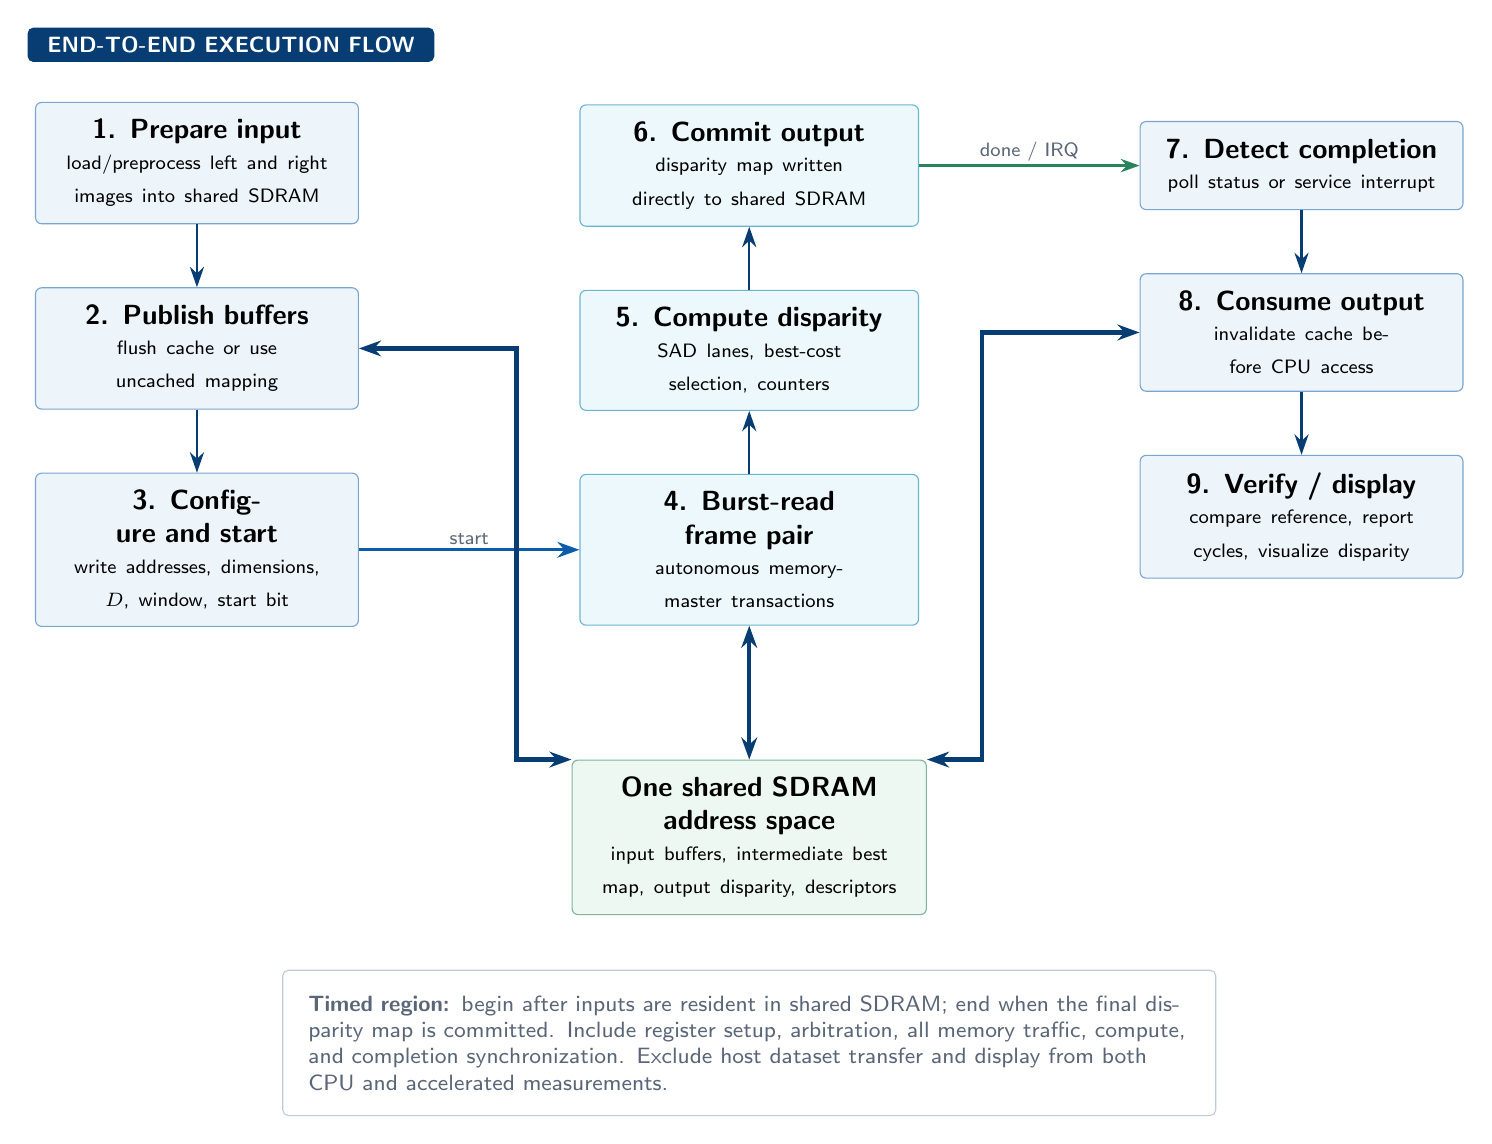
\begin{tikzpicture}[node distance=8mm and 15mm]
  \node[cpu, text width=35mm] (load) {\textbf{1. Prepare input}\\[-1pt]\scriptsize load/preprocess left and right images into shared SDRAM};
  \node[cpu, text width=35mm, below=of load] (flush) {\textbf{2. Publish buffers}\\[-1pt]\scriptsize flush cache or use uncached mapping};
  \node[cpu, text width=35mm, below=of flush] (config) {\textbf{3. Configure and start}\\[-1pt]\scriptsize write addresses, dimensions, $D$, window, start bit};

  \node[accel, text width=37mm, right=28mm of config] (read) {\textbf{4. Burst-read frame pair}\\[-1pt]\scriptsize autonomous memory-master transactions};
  \node[accel, text width=37mm, above=of read] (compute) {\textbf{5. Compute disparity}\\[-1pt]\scriptsize SAD lanes, best-cost selection, counters};
  \node[accel, text width=37mm, above=of compute] (write) {\textbf{6. Commit output}\\[-1pt]\scriptsize disparity map written directly to shared SDRAM};

  \node[cpu, text width=35mm, right=28mm of write] (done) {\textbf{7. Detect completion}\\[-1pt]\scriptsize poll status or service interrupt};
  \node[cpu, text width=35mm, below=of done] (invalidate) {\textbf{8. Consume output}\\[-1pt]\scriptsize invalidate cache before CPU access};
  \node[cpu, text width=35mm, below=of invalidate] (verify) {\textbf{9. Verify / display}\\[-1pt]\scriptsize compare reference, report cycles, visualize disparity};

  \draw[flow] (load) -- (flush);
  \draw[flow] (flush) -- (config);
  \draw[dataflow] (config.east) -- node[arrowlabel, above] {start} (read.west);
  \draw[flow] (read) -- (compute);
  \draw[flow] (compute) -- (write);
  \draw[returnflow] (write.east) -- node[arrowlabel, above] {done / IRQ} (done.west);
  \draw[flow] (done) -- (invalidate);
  \draw[flow] (invalidate) -- (verify);

  \node[memory, text width=39mm, below=17mm of read] (sdram) {\textbf{One shared SDRAM address space}\\[-1pt]\scriptsize input buffers, intermediate best map, output disparity, descriptors};
  \draw[bus] (flush.east) -| ([xshift=-7mm]sdram.north west) -- (sdram.north west);
  \draw[bus] (read.south) -- (sdram.north);
  \draw[bus] (invalidate.west) -| ([xshift=7mm]sdram.north east) -- (sdram.north east);

  \node[note, text width=112mm, below=9mm of sdram] (timing) {\textbf{Timed region:} begin after inputs are resident in shared SDRAM; end when the final disparity map is committed. Include register setup, arbitration, all memory traffic, compute, and completion synchronization. Exclude host dataset transfer and display from both CPU and accelerated measurements.};
  \draw[draw=line, rounded corners=2pt] ([xshift=-2mm,yshift=-2mm]timing.south west) rectangle ([xshift=2mm,yshift=2mm]timing.north east);

  \node[labeltag, anchor=south west] at ([xshift=-1mm,yshift=5mm]load.north west) {END-TO-END EXECUTION FLOW};
\end{tikzpicture}
\end{document}
